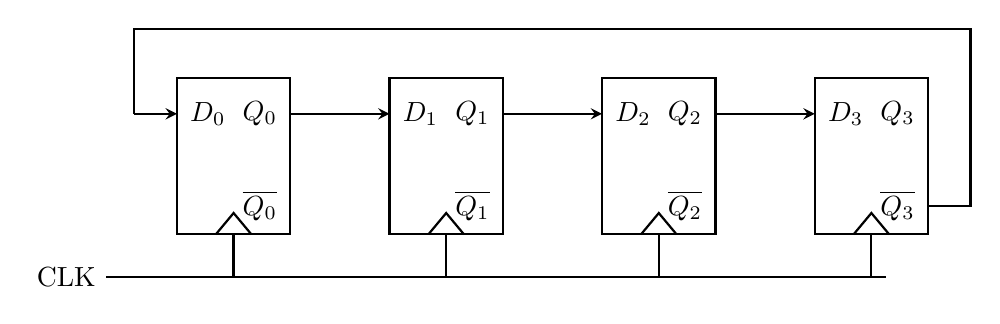
\begin{tikzpicture}[scale=0.9, >=stealth]
    \foreach \x/\i in {0/0, 3/1, 6/2, 9/3} {
        \draw[thick] (\x, 0) rectangle (\x+1.6, 2.2);
        \node[anchor=west] at (\x+0.05, 1.7) {$D_\i$};
        \node[anchor=east] at (\x+1.55, 1.7) {$Q_\i$};
        \node[anchor=east] at (\x+1.55, 0.4) {$\overline{Q_\i}$};
        \draw[thick] (\x+0.55, 0) -- (\x+0.8, 0.3) -- (\x+1.05, 0);
    }
    \draw[->, thick] (1.6, 1.7) -- (3.0, 1.7);
    \draw[->, thick] (4.6, 1.7) -- (6.0, 1.7);
    \draw[->, thick] (7.6, 1.7) -- (9.0, 1.7);
    \draw[thick] (10.6, 0.4) -- (11.2, 0.4) -- (11.2, 2.9) -- (-0.6, 2.9) -- (-0.6, 1.7);
    \draw[->, thick] (-0.6, 1.7) -- (0.0, 1.7);
    \draw[thick] (-1.0, -0.6) node[left] {CLK} -- (10.0, -0.6);
    \foreach \x in {0, 3, 6, 9} {
        \draw[thick] (\x+0.8, -0.6) -- (\x+0.8, 0.0);
    }
\end{tikzpicture}
